\chapter{Test} \label{ch:test}


\lipsum[1-3]

A table can look like \cref{tab:table}. A picture can be shown as in \cref{fig:dragonspaceship}.

\begin{table}[t!]
	\centering
	\caption{This is a caption.}
	\begin{tabular*}{\linewidth}{l @{\extracolsep{\fill}}cc}
		\toprule
		text & text & text \\
		\midrule
		 text & text & text \\
		 text & text & text \\
		\bottomrule
	\end{tabular*}
	\label{tab:table}  % label
\end{table}
\begin{figure}[t!] % "t" is for top
	\centering
	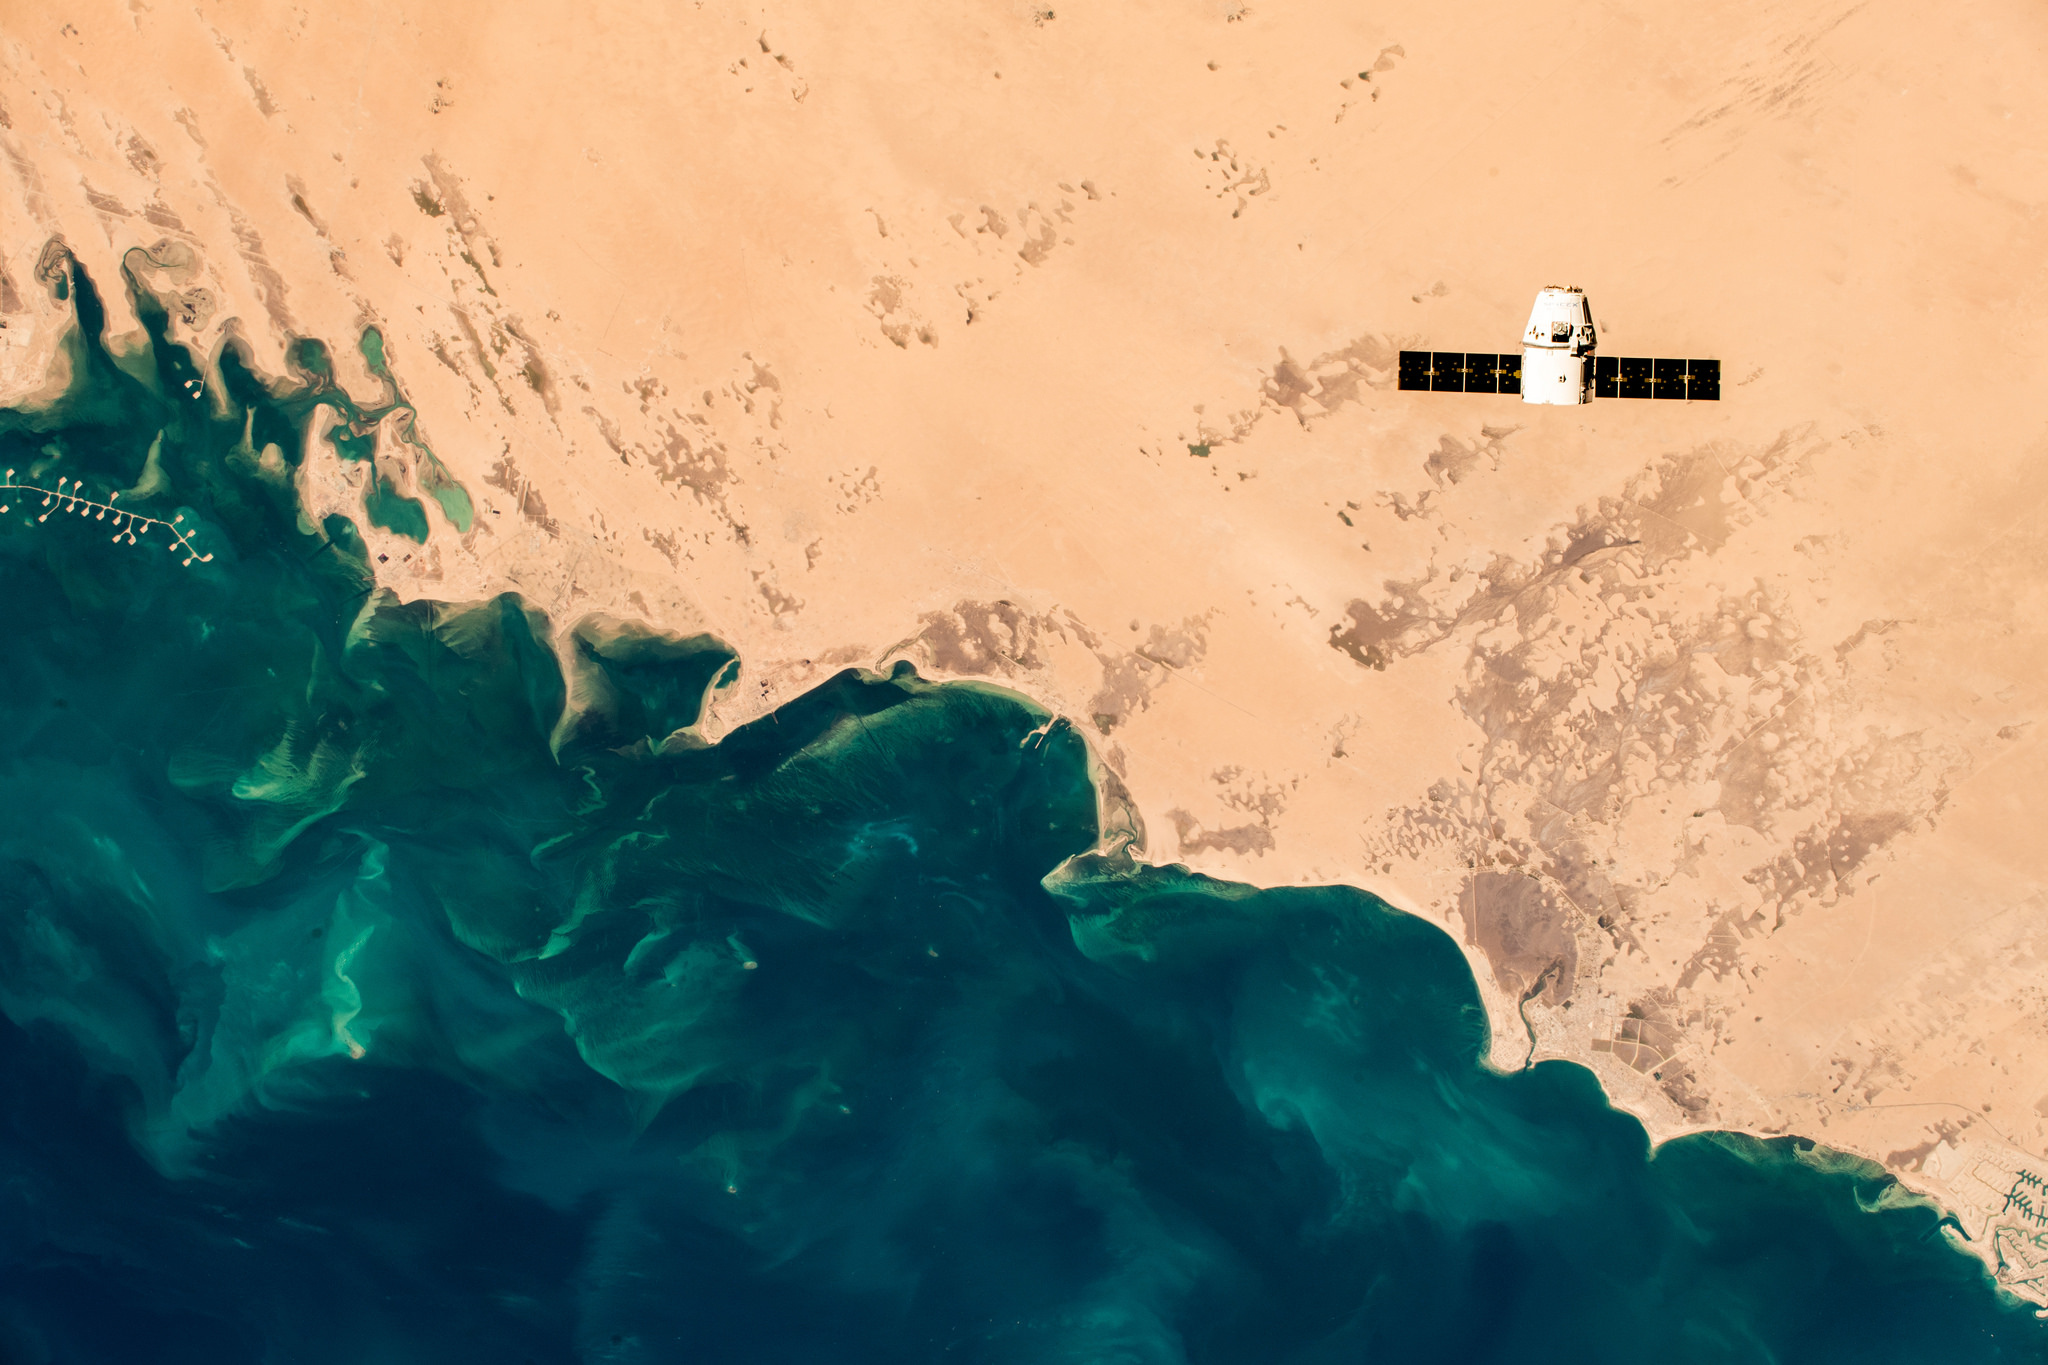
\includegraphics[width=0.8\linewidth]{figures/dragonSpaceship}
	\caption{This is a caption}
	\label{fig:dragonspaceship}
\end{figure}

Equations can be written as:
\begin{align}\label{equ:1}
A & = 1 +1 \\ \label{equ:2}
C & = \dfrac{3}{x} 
\end{align}
where \cref{equ:1} is equation 1. The package cleveref is here used. A list of useful \LaTeX packages is available at \url{https://blog.martisak.se/2020/05/03/top-ten-latex-packages/}.
